% Combined and expanded Data Descriptor paper for the DAS dataset

\documentclass[11pt]{article}

% Packages
\usepackage{graphicx}
\usepackage{authblk}
\usepackage{amsmath}
\usepackage[a4paper,margin=2.2cm]{geometry}
\usepackage{hyperref}
\usepackage{caption}
\usepackage{float}
\usepackage{booktabs}
\usepackage[numbers]{natbib}

\usepackage{array,tabularx,booktabs,siunitx,ragged2e}
\newcolumntype{Y}{>{\RaggedRight\arraybackslash}X} % X con alineación raggedright
%\usepackage{booktabs}
%\usepackage{tabularx}
%\usepackage{siunitx}

\usepackage{wrapfig}%,graphicx,hyperref}

\graphicspath{{./figures/}{./results/}}

\usepackage[caption=false,font=normalsize,labelfont=sf,textfont=sf]{subfig}

\newcommand{\mysubfigure}[3]{%
    \subfloat[#2]{\includegraphics[width=#1]{#3}}%
}
\captionsetup[subfloat]{font=footnotesize} % Or small/tiny
\captionsetup[subfloat]{font=scriptsize} % Or small/tiny

\usepackage[dvipsnames]{xcolor}
\definecolor{darkgreen}{rgb}{0.0, 0.5, 0.0}
\definecolor{brown}{rgb}{0.6, 0.3, 0.0}
\definecolor{darkbrown}{rgb}{0.4, 0.2, 0.0}

% todonotes definitions
\usepackage{todonotes}

\newcommand{\todojmg}[1]{\todo[author=JMG,inline,color=blue!30]{#1}}
\newcommand{\tododpp}[1]{\todo[author=DPP,inline,color=orange!30]{#1}}
\newcommand{\todojtn}[1]{\todo[author=JTN,inline,color=yellow!30]{#1}}
\newcommand{\todosepc}[1]{\todo[author=SEPC,inline,color=purple!30]{#1}}
\newcommand{\todosml}[1]{\todo[author=SML,inline,color=cyan!30]{#1}}
\newcommand{\todomgh}[1]{\todo[author=MGH,inline,color=red!30]{#1}}
\newcommand{\rojo}[1]{\textcolor{red}{#1}}
\newcommand{\azul}[1]{\textcolor{blue}{#1}}

% and their extensions so you won't have to specify these with
% every instance of \includegraphics
\DeclareGraphicsExtensions{.pdf,.jpeg,.png}

\usepackage{hyperref}
\usepackage{hyperxmp}
\hypersetup{
%% ps2pdf,                %%% hyper-references for ps2pdf
bookmarks=true,%                   %%% generate bookmarks ...
bookmarksnumbered=true,            %%% ... with numbers
hypertexnames=false,               %%% needed for correct links to
%%% figures!!!
% hypertexnames=true,               %%% needed for correct links on pagebackrefs!!!
breaklinks=true,                   %%% breaks lines, but links are very small
% pagebackref=true,
% linktocpage=true,                 %%% enlace en el numero de página.
linktoc=all,
colorlinks=true,
linkcolor=blue,
citecolor=blue,
urlcolor=blue,                     %%% texto  con color (further
%%% modified in myconfig.tex)
% linkbordercolor={0 0 1},           %%% blue frames around links
pdfborder={0 0 112.0},              %%% border-width of frames
hyperfootnotes=false
}                        %%% will be multiplied with 0.009 by ps2pdf

% Title and authors
\title{A distributed acoustic sensing dataset for vessel detection and localization in submarine cable protection tasks}

\author[1]{Erick Eduardo Ramirez-Torres}
\author[1]{Sira Elena Palazuelos-Cagigas}
\author[1]{Javier Macias-Guarasa}
\author[1]{Daniel Pizarro}
\author[2]{Javier Tejedor}
\author[1]{Sonia Martin-Lopez}
\author[1]{Miguel Gonzalez-Herraez}
\author[3]{Roel Vanthillo}

\affil[1]{Universidad de Alcal\'a, Departamento de Electr\'onica, Alcal\'a de Henares, Spain}
\affil[2]{Universidad San Pablo-CEU, Boadilla del Monte, Spain}
\affil[3]{Marlinks, Leuven, Belgium}

\date{}


\begin{document}
\maketitle


\begin{abstract}
% Recent incidents of accidental damage and suspected sabotage to submarine telecommunication and power cables in regions such as the Baltic Sea have underscored the vulnerability of these infrastructures and the urgent need for continuous monitoring solutions. Distributed Acoustic Sensing (DAS) applied to submarine optical fiber cables enables continuous, wide-area monitoring of underwater acoustic activity, providing a powerful tool for maritime surveillance and ocean observation.

% We present here the rigorously curated \texttt{Marlinks-NS} Distributed Acoustic Sensing (DAS) dataset that provides the first large-scale, open collection of DAS measurements acquired from a submarine telecommunication cable specifically aimed at submarine cable protection tasks. The release data defines two machine learning tasks (ML), for both vessel detection and vessel distance estimation tasks, enabling reproducible ML studies under realistic marine conditions.

% The dataset consists of over $74,000$ preprocessed and labeled data frames derived from more than ten days of continuous recording on a $28\,km$ buried submarine optical fiber cable in the southern North Sea. Each frame data contains energy values computed in $100$ logarithmically spaced frequency bands, accompanied by anonymized synchronized vessel metadata (distance to the cable, type, beam, and length) extracted from Automatic Identification System (AIS) information. The release includes a complete description of the data structure, processing workflow, and example code for loading and manipulating the data. By providing a machine-learning-ready representation of DAS signals, the \texttt{Marlinks-NS DAS} dataset aims to serve as a reference resource for developing and benchmarking algorithms for vessel detection, classification, and localization using submarine fiber infrastructures applied to submarine cable protection tasks.

Recent incidents of accidental damage and suspected sabotage to submarine telecommunication and power cables, particularly in the Baltic Sea, have underscored their vulnerability and the need for continuous monitoring solutions. Distributed Acoustic Sensing (DAS) applied to submarine optical fiber cables enables wide-area, real-time monitoring of underwater acoustic activity, providing a promising tool for maritime surveillance and cable protection.

We present the \texttt{Marlinks-NS} DAS dataset, a large-scale, openly available collection of submarine DAS measurements specifically curated for cable protection research. The dataset defines two machine learning tasks (vessel detection and vessel distance estimation) allowing reproducible studies under realistic marine conditions.

The dataset contains over $74,000$ preprocessed and labeled data instances from more than ten days of continuous recording along a relevant segment in a $28\,km$ buried fiber optic cable in the North Sea. Each instance includes 100-band spectral energy features and anonymized vessel metadata from the Automatic Identification System (AIS). The dataset, processing workflow, and example code together provide a benchmark for developing and validating DAS-based methods for vessel monitoring and submarine cable protection.
\end{abstract}


\section{Background \& Summary}

Submarine cables are vital for global communication and power transmission but remain vulnerable to accidental damage and sabotage, with recent severe examples in the Baltic Sea with, for example, the damage to the EstLink2 power cable~\cite{navalnews_estlink2_2024}, and the C-Lion1 communication cable~\cite{euromaidan_baltic_2025}, suspected of sabotage and linked to geopolitical tensions.

Distributed Acoustic Sensing (DAS) technology allows repurposing of standard optical fibers into dense acoustic sensor arrays capable of capturing vibrations and strain over tens of kilometers. In the context of submarine cables, this capability opens the path to a cost-effective means of monitoring marine activity to prevent accidental damage or sabotage. Unlike radar or satellite-based systems, DAS provides continuous, real-time coverage, is largely unaffected by lighting or weather conditions, and does not depend on cooperative identification systems such as the Automatic Identification System (AIS).

Publicly available datasets enabling the development of data-driven algorithms for DAS-based vessel detection are scarce. Existing works are often limited in scale, or lack of properly labeled metadata that allow research in Artificial Intelligence Machine Learning strategies (AI/ML). This scarcity is particularly severe in specialized environments like submarine cables. Initiatives such as PubDAS~\cite{pubDAS2023} (the first large-scale open-source repository for DAS data) have demonstrably accelerated research by providing multiple experiment datasets for benchmarking and algorithm development. So, the number of publicly available resources in submarine environments are very limited. Some relevant examples in this scenario are:

\begin{itemize}
  \item The DAShip dataset, by Huang et al.~\cite{Huang2025DAShip} (available at \cite{DAShip2025}).
  \item The MARS DAS experiment dataset by Cheng et al.~\cite{cheng2021utilizing} (available at~\cite{cheng2020mbari_das_data} with a \href{https://github.com/njlindsey/Photonic-seismology-in-Monterey-Bay-Dark-fiber1DAS-illuminates-offshore-faults-and-coastal-ocean}{repository at Github}).
  \item The MEUST DAS dataset by Sladen et al.~\cite{sladen2019distributed} (available at~\cite{sladen2019meust_km3net_das}).
  \item The HCMR+NESTOR+MEUST DAS datasets by Lior et al.~\cite{lior2021detection} (available at~\cite{lior2021detection_dataset}).
  \item The DAS4Microseism dataset, by Taweesintananon et al.~\cite{Taweesintananon2023} (available at~\cite{VPRD2H_2022}).
  \item The OOI Regional Cabled Array (RCA) Dataset, by Lipowsky et al.~\cite{shi2025multiplexed} (available at \cite{lipovsky2024rapid_das_ooi} with a \href{https://github.com/uwfiberlab/OOI_DAS_2024}{source code repository at GitHub}).
  \item The Valencia-IslaLink DAS dataset, by Spica and Gaite, which is distributed within PubDAS~\cite{pubDAS2023}.%, recorded in a telecommunication fiber-optic cable operated by IslaLink Holding Iberia S.L. and connecting Valencia to Palma de Mallorca. Data corresponds to the first $50\,km$ of the cable (the first $~10\,km$ are on land and the remaining corresponds to a buried cable about $1\,m$ below the Mediterranean seabed). 7 days of continuous data are available (from September $1^{st}$ to $7^{st}$ 2023).
  \item The Yellow River Delta Dataset, by Song et al.~\cite{song2024near} (available at~\cite{song_2024_dataset}).
\end{itemize}

\begin{table*}[t]
\centering
\footnotesize
\setlength{\tabcolsep}{3pt}     % compacto
\renewcommand{\arraystretch}{1.15}
\caption{Summary of publicly released DAS datasets cited in this work, including application domain, fiber length, dataset size, sampling frequency, and recording period. Fields marked as \textit{TBD} should be completed using the information in the corresponding bibliographic sources.}
\label{tab:das_datasets}
\begin{tabularx}{\linewidth}{
  >{\RaggedRight\arraybackslash}p{2.8cm}|  % Dataset
  >{\RaggedRight\arraybackslash}p{3.3cm}|  % Domain
  >{\RaggedRight\arraybackslash}p{2.0cm}|  % Fiber length
  >{\RaggedRight\arraybackslash}p{2.0cm}|  % Dataset size
  >{\RaggedRight\arraybackslash}p{1.8cm}|  % Sampling frequency
  Y                                        % Notes
}
\hline
\textbf{Dataset} &
\textbf{Application domain} &
\textbf{Fiber length} &
\textbf{Dataset size} & \textbf{Sampling frequency and gauge length} &
\textbf{Annotation}\\
\hline
DAShip~\cite{Huang2025DAShip} &
Wake ship detection and vessel speed/angle classification &
8.5\,km &
55875 ship passing events above the cable &
10\,Hz GL=4\,m&
Annotated using AIS guidance (for the three binary classification tasks)\\
\hline
MARS DAS experiment~\cite{cheng2021utilizing,cheng2020mbari_das_data} &
Ocean dynamics \& subsurface characterization &
51\,km &
4 days, 3.2TB &
250\,Hz GL=10\,m&
No labeling provided \\
\hline
MEUST~\cite{sladen2019distributed,sladen2019meust_km3net_das} &
Seismic monitoring &
41.5\,km &
6 days &
1\,kHz GL=19.2\,m &
No labeling provided \\
\hline
HCMR+ NESTOR+ MEUST~\cite{lior2021detection,lior2021detection_dataset} &
Seismic monitoring &
13.2\,km, 26.2\,km and 44.8\,km &
1 day (68 GB), 7 days (740 GB), 20 days (16 TB) &
Between 100\,Hz and 500\,Hz. GL=19.2\,m/10\,m &
No labeling provided \\
\hline
DAS4Microseism~\cite{Taweesintananon2023,VPRD2H_2022} &
Ocean dynamics \& subsurface characterization &
120\,km &
44 days &
50\,Hz GL=8-16\,m&
No labeling provided \\ %; fiber buried 0--2\,m below the seafloor \\
\hline
OOI RCA~\cite{shi2025multiplexed,lipovsky2024rapid_das_ooi} &
Seismic monitoring &
~95\,km &
4 days, 2.4TB &
200\,Hz GL=40.852\,m &
No labeling is provided\\
\hline
Valencia~\cite{pubDAS2023} &
Submarine monitoring vibrations (telecommunication cable) &
$\sim$50\,km (first $\sim$10\,km on land) &
7 days, 3TB &
250\,Hz GL=30.4\,m&
No labeling provided \\ %; fiber buried $\sim$1\,m below the seabed in the submarine section\\
\hline
Yellow River Delta~\cite{song2024near,song_2024_dataset} &
Nearshore ocean current monitoring &
10\,km &
25 days &
50\,Hz  GL=5\,m&
Provide labels for wind speed and tidal data \\
\hline\bottomrule
\end{tabularx}
\end{table*}


Table~\ref{tab:das_datasets} shows the relevant characteristics of each of them. Except for DAShip, all these datasets are oriented to applications in the seismic and ocean monitoring domain without explicit labeling information that can support experimental work in vessel detection and localization. DAShip is a large-scale, annotated dataset collected for the specific purpose of marine vessel detection. It comprises 55,875 ship-related event segments, captured on a submarine fiber-optic cable, $8.5\,km$ long, with a maximum depth of $13\,m$ along the cable deployment (according to GEBCO bathymetry information~\cite{gebco2024}). It is oriented to the detection of vessel passages right  above the fiber optic cable, using image classification algorithms to identify the ships' wakes, to that it cannot be used for preventive submarine cable protection, as the detection happens when the vessel is already above the cable. Another limitation is that the data has been downsampled to $10\,Hz$, which has two main issues: first, this reduced bandwidth does not allow to exploit vessel acoustic signatures, which exhibits relevant frequency components in higher frequencies~\cite{Rivet_2021,Thiem_2023}; and second, it will be more affected by low frequency noise from temperature drift, and, more importantly, from the effect of sea waves and marine currents.

We can mention other properly labeled recent datasets which address event classification tasks, but in terrestrial domains, such as that by Tomasov et al.~\cite{tomasov2025comprehensive} that presented a fully labeled DAS dataset, including band-limited feature vectors. The fiber was $1663\,m$ long, and was buried $1\,m$ below the surface around a rectangular area in an university campus. The selected events included walking, running, longboarding, and driving, as well as potential security-related events like fence climbing, fiber manipulation, and opening/closing of manholes.

The \texttt{Marlinks-NS DAS} dataset we present in this paper addresses the lack of publicly accessible, well-annotated DAS data aimed at submarine cable protection applications, by defining two AI/ML tasks, one for vessel detection, and another for vessel distance estimation. The dataset provides a large-scale, machine-learning-ready collection of preprocessed spectral features and vessel metadata derived from a ten-day continuous recording campaign on a submarine cable. It comprises $74,771$ data instances (feature vectors) computed at $250$ channels in a relevant fiber optic range, each containing energy values in $100$ logarithmically spaced frequency bands, together with synchronized vessel distance % and vessel presence
labels, plus anonymized vessel related information obtained from AIS (type, beam, and length). By releasing this curated dataset, we aim to promote transparency and reproducibility in AI/ML-based DAS research while enabling the scientific community to benchmark vessel detection and localization algorithms under realistic conditions. Additionally, accompanying code has been made available at \url{https://github.com/UAH-PSI/das-vessel-detection} to ease the community in this research area to quickly engage in experimental work.


\section{Methods}
\label{sec:methods}

The processing pipeline we applied for the generation of the dataset is shown in Fig.~\ref{fig:architecture}, to provide a full reference about the data curation process. All the relevant methods and modules are described in the following subsections.

\begin{figure}[H]
  \centering
  \includegraphics[width=\textwidth]{system-architecture-v7.png}
  \caption{Dataset curation and processing pipeline, covering DAS acquisition and raw signal preprocessing; spectral feature extraction; metadata (AIS, geographical location and bathymetry) processing, synchronization and label generation; and cross validation partitioning.}
  \label{fig:architecture}
\end{figure}


\subsection{DAS interrogator: Acquisition Method and Setup}
\label{sec:acquisition-method}

The submarine fiber optic cable was interrogated using a phase-sensitive Optical Time Domain Reflectometry ($\phi$-OTDR) system. This approach uses a narrow-linewidth, highly coherent laser that emits short optical pulses into the fiber core, where microscopic refractive index variations act as Rayleigh scatterers. The backscattered signal from each pulse carries amplitude and phase information that varies with longitudinal deformation in the fiber, that can be related to vibrations and acoustic disturbances in the cable vicinity. By measuring phase differences between consecutive backscatter traces, dynamic strain variations can be reconstructed continuously along the entire length of the fiber.

The DAS data were recorded using an Alcatel OptoDAS interrogator~\cite{OptoDAS} connected to a $28\,km$ ocean-bottom fiber-optic cable originally deployed for power cable monitoring. The cable lies buried between $1.4-7.2\,m$ below the seafloor, offshore Zeebrugge (Belgium) in the North Sea, as shown in Fig.~\ref{fig:geographical-location}. The interrogator, located off-shore, employs optical pulse-compression reflectometry, that enables distributed vibration sensing over tens of kilometers with meter-scale spatial sampling while mitigating fading effects due to low-intensity points in the Rayleigh pattern \cite{gabai2016sensitivity, Zou_2015, Waagaard_2021}.  with a gauge length of $L=10.21\,m$, generating $2774$ raw spatial channels. The raw differential-phase signals were sampled at $f_s=3125\,Hz$.
\begin{figure*}[hbtp]
  \centering
  \mysubfigure{0.292\textwidth}{Regional map.}{area-location-map-google-earth-trimmed.png}
  \label{fig:regional-map}
  ~%add desired spacing between images, e. g. ~, \quad, \qquad,
  % \hfill etc.
  % (or a blank line to force the subfigure onto a new line)
  \mysubfigure{0.290\textwidth}{Local map showing cable (red line).}{local-map-google-earth.png}
  \label{fig:local-map}
  ~
  \mysubfigure{0.378\textwidth}{Local map showing cable (red line) and  bathymetry.}{E4_2022_mean-ocean-paper-trimmed.png}
  \label{fig:bathymetry-map}
  \caption{General location and bathymetry (cable location has been displaced for security considerations), from~\cite{ramirez2025vessel}.}
  \label{fig:geographical-location}
\end{figure*}



\subsection{DAS Preprocessing}
\label{sec:signal preprocessing}

In this stage, the raw differential-phase time series generated by the DAS interrogator are converted to strain. This procedure is very closely related to the interrogator design and characteristics, so that the corresponding modules are mainly provided by the cable operator. The operations carried out are:

\begin{itemize}
  \item Amplitude scaling, to ensure consistent amplitude levels in $rad/m/s$.
  \item Spike detection and removal.
  \item Phase unwrapping to remove $2\pi$ discontinuities.
  \item Temporal integration and scaling to recover strain values in $m/m$.
\end{itemize}

This process ensures consistent, and physically interpretable strain signals across all channels.

Figs.~\ref{fig:energy-dt-map}.a+b and~\ref{fig:strain-silence}.a+b show two examples of the generated strain signals for scenarios with a vessel nearby or in the absence of nearby vessels, respectively.



\subsection{Metadata Processing: AIS Data Processing}
\label{sec:ais-data-processing}

\todojmg{Erick, revisa please las estadísticas de AIS que pone aquí.}

The AIS data provided by the cable operator included vessel identifiers (MMSI), timestamps, coordinates, course, and speed for 745 unique vessels with 64,417 position reports. A relevant problem when using AIS data is the unpredictable and typically low position update rates~\cite{emmens2021promisesAIS}. A detailed analysis on our DAS data showed that $88\%$ of vessels reported positions only every 1 to 3 minutes, which may imply a significant positional uncertainty. To overcome this issue, we applied a linear interpolation between consecutive reported positions at $1\,Hz$ position update rate. %, discarding trajectories with gaps exceeding $60$ minutes.
We did not have the possibility of a direct quantitative validation on the precision of this simple interpolation approach (provided AIS data was the only available source of vessel positioning), but the good results obtained (see Section~\ref{sec:technical validation}) served us a kind of ``indirect validation'', so that we did not require to apply more sophisticated interpolation methods~\cite{guo2021improved}.

After the interpolation process, we had over $1,200,000$ AIS position entries, which we further enriched with web-scrapped additional AIS metadata (namely, vessel type, length and beam) that can be useful in further studies or AI/ML tasks requiring information related to vessel type and size.


\subsection{Metadata Processing: Geographical+Bathymetry Data Processing}
\label{sec:geospatial-tagging}

In our DAS context, geospatial tagging refers to the process of assigning precise geographical coordinates, and depth or elevation to each sensed position along the fiber optic cable. In DAS applications, accurate geospatial tagging is crucial because it relates the distributed acoustic measurements to their exact physical locations along the fiber, enabling spatially consistent signal interpretation, correlation with environmental and bathymetric data, and the development of position-dependent models for event localization and propagation analysis~\cite{holman2025}.

In our dataset, each DAS sensing position along the selected cable segment was assigned precise geospatial coordinates combining information from the data owner (that provided the reference longitude and latitude of the submarine cable route), and the depth information extracted from the EMODnet bathymetry service~\cite{emodnet2024}. This combination resulted in a complete set of geospatial attributes (longitude, latitude, depth) for all the DAS channels, which provides a fundamental reference the in our geographically informed ML tasks using the \texttt{Marlinks‐NS DAS} dataset.


\subsection{ML Tasks and Data Balance Considerations}
\label{sec:ml-tasks}

In ML applications, maintaining a balanced dataset helps to ensure unbiased model training and fair performance evaluation. For classification tasks, balance in the number of samples per class prevents the model from favoring dominant categories. For regression tasks, an even distribution of target values enables the model to learn the underlying functional relationships for the full data range, rather than overfitting to the most densely sampled regions. However, achieving such balance is often difficult in real-world scenarios, where natural or operational processes generate highly uneven data distributions, which is usually the case in AI/ML-based DAS applications..

The \texttt{Marlinks-NS DAS} dataset has been designed to support two complementary machine learning (ML) tasks related to vessel monitoring for submarine cable protection. The first task, \emph{vessel detection}, is formulated as a binary classification problem that is oriented to discriminate whether there is a vessel closer than a given distance threshold to the cable. The second task, \emph{distance estimation}, is defined as a regression problem in which the model aims to predict the distance between the cable and the nearest vessel. In both cases the required labeling information is derived from the synchronized AIS data.

\begin{figure}[hbtp]
  \centering
  \includegraphics[width=\columnwidth]{class-distribution/class_balance_1000_2000_3000_4000_5000_ship_channel.jpg}
  \caption{Number of data frames corresponding to vessels located at different distance ranges from the cable.}
  \label{fig:data-balance}
\end{figure}

To assess whether both tasks are representative, and evaluate their statistical balance, a detailed analysis of the vessel distance distribution along the monitored cable was performed. Initial inspection of the ten-day continuous recording revealed strong spatial distribution nonuniformity. Fig.~\ref{fig:data-balance} shows, as a function of the channel position along the cable length, the number of 10-second data frames that corresponds to a situation in which there is a vessel at different distance ranges. From the figure we can identify a cable section around $16\,km$ (channel 1565) that exhibits a relevant increase in the number of available data frames with vessels closer to the cable than, for example, $1000\,m$ or $2000\,m$, which are reasonable thresholds for the vessel detection task. As an example of the rationale for such ``reasonable threshold'' statement, a Spanish company monitoring submarine cables with AIS, establishes a $1000\,m$ distance threshold to trigger enhanced vessel tracking to assess potential threats to the cable.

This region corresponds to the location of the cross between the submarine cable and a dredged channel (approximately $20\,m$ deep) providing harbor access, which is consistent with the higher density of vessels shown in Fig.~\ref{fig:data-balance}. So, given this spatial data distribution, we selected a contiguous cable range of $2553\,m$,  corresponding to a subset of $N_{channels}=250$ equally spaced spatial channels located between $14707\,m$ and $17260\,m$ from the interrogator. This segment exhibits a clear unbalance between the ``vessel-nearby'' and ``no-vessel-nearby'' classes (e.g. $22347$ vs. $52424$ for the $1000\,m$ distance threshold), but provides a reasonable availability of data samples for both of them. %, as well as a broad dynamic range of distances suitable for regression.
The \texttt{Marlinks-NS DAS} dataset contains full data for this cable segment, and there is no other better fiber range in what respect to data unbalance and class-wise data availability.% Fig.~\ref{fig:histogram-distance} shows the distribution of data frames as a function of the \textit{minimum} distance of \textit{any} vessel to the cable, which shows the expected behavior (considering that it is not the distribution of vessel distances).

% \begin{figure}[hbtp]
%   \centering
%   \includegraphics[width=.75\columnwidth]{balance/histogram_distance.png}
%   \caption{Histogram of data frames available as a function of the \textit{minimum} distance of \textit{any} vessel to the cable.}
%   \label{fig:histogram-distance}
% \end{figure}

Finally, to give an idea on the distribution of vessel types, Fig.~\ref{fig:piano-distance-by-type} shows the distribution boxplots of minimum distances by vessel types, in which the top numbers ($n=\dots$) state the number of examples of each vessel type in the dataset.

\begin{figure*}[hbtp]
  \centering
  \includegraphics[width=\columnwidth]{balance/boxplot_by_type.png}
  \caption{Histogram of data frames available as a function of the \textit{minimum} distance of \textit{any} vessel to the cable, per vessel type.}
  \label{fig:piano-distance-by-type}
\end{figure*}

\begin{figure}[htbp]
  \centering
  \includegraphics[width=\textwidth]{strain-silence+spectrum.png}
  \caption{(a) Strain signal when no vessel is nearby the cable (it corresponds to the right dashed square in Fig.~\ref{fig:energy-dt-map}): Filtered strain signal at $15.4\,km$ in the time interval of the right red dashed square in Fig.~\ref{fig:energy-dt-map}. (b) Filtered strain data as a function of time and distance corresponding to the right red dashed square in Fig.~\ref{fig:energy-dt-map}, time synchronized with Fig.~\ref{fig:strain-silence}.a. (c) Long term averaged strain power spectrum plots (expressed in dBs) for strain measurements for vessels closer than $1000\,m$ to the cable (\textcolor{darkgreen}{\textrm{Vessels 1000m}} trace), and vessels further than $3000\,m$ (\textcolor{darkbrown}{\textrm{Noise 3000m}} trace).}
  \label{fig:strain-silence}
\end{figure}

\subsection{Feature Extraction}
\label{sec:feature extraction}

In this work we carried out a data-driven methodology to decide on the feature vector composition, informed by available AIS data, and fully described in~\cite{ramirez2025vessel}. The main idea here is that we analyzed strain long-term  spectral averages of both vessel and background noise and found out that there were promising spectral differences between both cases in the range between $4\,Hz$ and $100\,Hz$. Additionally we discovered a strong spectral peak located at $100\,Hz$, with harmonics at its integer multiples, and one subharmonic at $50\,Hz$, probably due to the interference generated by rotating mechanical systems or electric noise in the interrogator environment. Fig.~\ref{fig:strain-silence}.c shows strain long-term spectral averages (in dBs) for the case of vessels closer than  $1000\,m$ to the cable (\textcolor{darkgreen}{\textrm{Vessels 1000m}} trace) and for the case of vessels further than $3000\,m$ (\textcolor{brown}{\textrm{Noise 3000m}} trace).



The strain signal for each channel was first segmented into non-overlapping windows of length $T_\omega=10\,s$, to which we apply a ¿HAMMING WINDOW? to avoid spectral leakage. The window size was selected to allow for a reasonable resolution in the few-Hz frequency range, considering that we wanted to avoid low frequency noise (mainly from temperature variations and surface waves). Thus, for each 10-second windows we run a Fast Fourier Transform (FFT) analysis to provide spectral components for the feature vector build-up, selecting an initial bandwidth between $4\,Hz$ and $100\,Hz$.

The feature vector is then generated from the FFT values, so that each 10-second window is represented by $N_{bands}=100$ logarithmically spaced band-energy features within the 4--100~Hz range, excluding the 49--51~Hz and 98--100~Hz intervals. The logarithmic frequency mapping was designed to equalize the required spectral resolution, allocating more spectral FFT coefficients in the lower frequency region (the specific frequency band limits can be found in \href{https://github.com/UAH-PSI/das-vessel-detection/blob/main/data/fbands.csv}{the GitHub repository}).

The mathematical details for the feature extraction calculation follow. We first assume that $x_c^{(n)}[m]$ denote the discrete version of the $n^{th}$ windowed strain signal corresponding to channel $c$ starting at $n·T_\omega$ seconds, with $n\nobreak=0, 1, \dots, N_{windows}-1$; and that $X_c^{(n)}[k]$ is the $N_{\mathrm{FFT}}$-point FFT of $x_c^{(n)}[m]$, with $c=0,1,\dots N_{channels}-1$ being $N_{windows}$ and $N_{channels}$ the number of available windows and available channels, respectively. Each spectral band $b = 0, 1, \dots, N_{bands}\text{-}1$ is defined by its FFT-bin limits $\big[k_b^{-},\, k_b^{+}\big]$, where $0 \le k_b^{-} \le k_b^{+} < N_{\mathrm{FFT}}$.
From these definitions, the spectral energy of band $b$ for window $n$ of channel $c$ is computed as:
\begin{equation}
E_c^{(n)}[b] = \sum_{k = k_b^{-}}^{k_b^{+}} \big| X_c^{(n)}[k] \big|^2.
\end{equation}

Finally, the feature vector corresponding to $x_c^{(n)}[m]$ will be $\mathcal{E}_c^{(n)}=\left[ E_c^{(n)}[0], E_c^{(n)}[1], \dots, E_c^{(n)}[N_{bands}-1] \right]$, which corresponds to the $N_{windows}\times \left( N_{channels}\times N_{bands}\right)$ values available in the public dataset.

\todojmg{Erick, please verifica que las ecuaciones son las que tú usas.}
\begin{figure}[htbp]
  \centering
  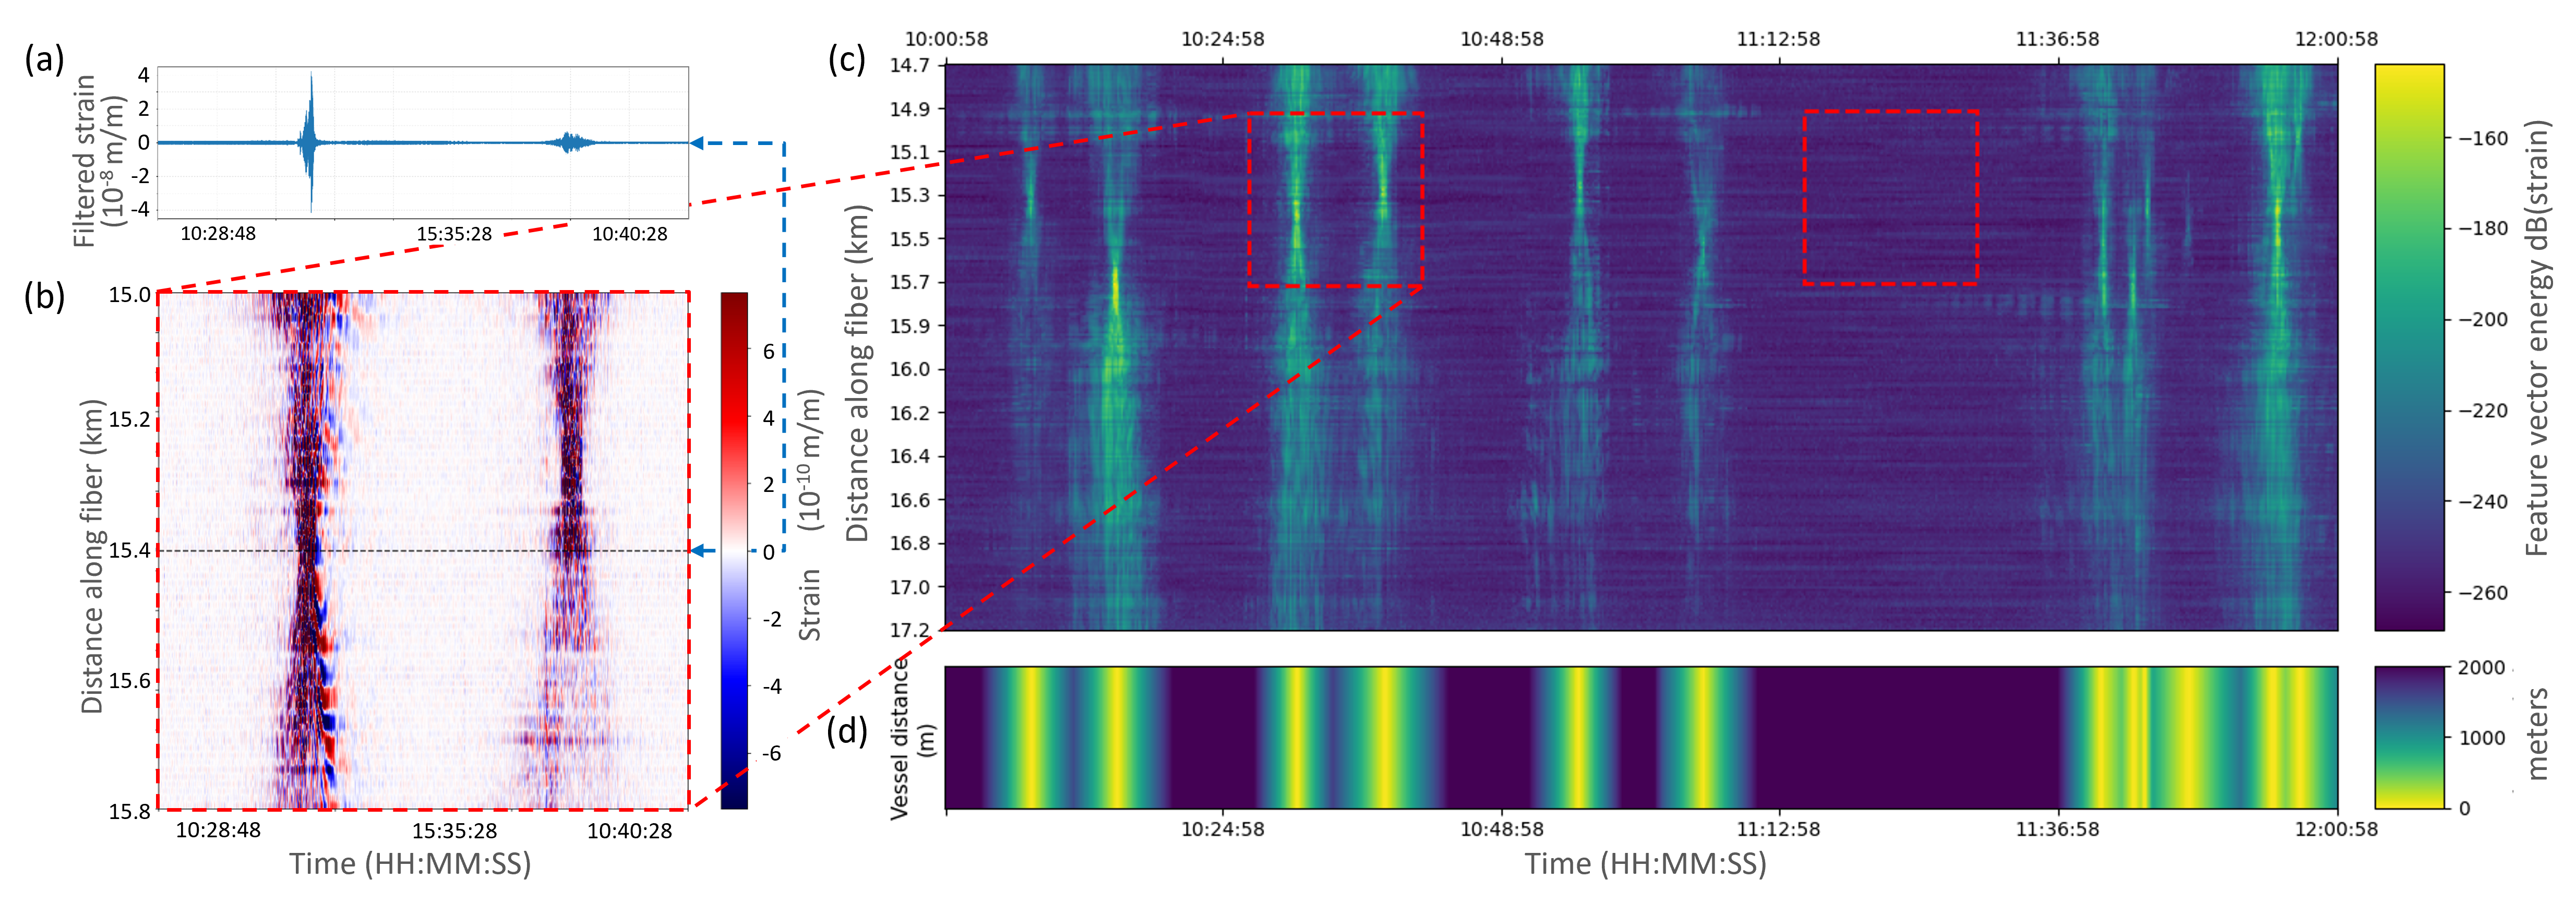
\includegraphics[width=\textwidth]{dt-full.png}
  \caption{(a) Raw strain signal sensed at $15.4\,km$ in the time interval of the red dashed square in Fig.~\ref{fig:energy-dt-map}.d. (b) Filtered strain signal ($4\,Hz$ to $98\,Hz$, excluding the $(49-51)\,Hz$) corresponding to the raw signal in Fig.~\ref{fig:energy-dt-map}.a and time-synchronized with it. (c) Filtered strain data as a function of time and distance along the cable corresponding to the red dashed square in Fig.~\ref{fig:energy-dt-map}.d, time synchronized with Figs.~\ref{fig:energy-dt-map}.a and~\ref{fig:energy-dt-map}.b. (d) Feature vector energy (in dBs) as a function of time and distance along the cable. (e) Distance from cable to nearest vessel (in meters), time-synchronized with Fig.~\ref{fig:energy-dt-map}.d.}
  \label{fig:energy-dt-map}
\end{figure}


\subsection{Data Synchronization and Labeling}
\label{sec:ais data and label generation}

Time synchronization between the DAS signals and the interpolated AIS information is carried out as a required step before data labeling is carried out. The interpolated AIS positions are then used to continuously compute the shortest distance between each vessel and every DAS sensing point. These distance values are considered within each 10-seconds strain signal window to determine the minimum vessel to cable distance used as the primary label for the ML tasks. This synchronization process ensures that all DAS feature vectors are associated with consistent, temporally aligned vessel metadata.

The closest distance continuous variable supports regression tasks directly as \texttt{Vessel distance labels}, or can be converted into \texttt{vessel detection labels} for the classification task, by simply applying user-defined distance thresholds.


\section{Data Records}
\label{sec:data records}

The dataset is publicly available on Zenodo~\cite{ramirez2024dasvesseldataset}, and to simplify its distribution, all the data are stored in a \texttt{hdf5} archive (14 GB in size) with the following structure (summarized in Table~\ref{tab:dataset-content}):
\begin{itemize}
  \item \texttt{X}: A 3D NumPy array of shape {($N_{windows}$, $N_{channels}$, $N_{bands}$)}, containing the feature vectors. XXXXXXXXXXX WHICH UNITS?
  \begin{itemize}
    \item \textbf{{$N_{windows}=74771$}}: number of non-overlapped 10-seconds signal windows analyzed along the full recording period.
    \item \textbf{{$N_{channels}=250$}}: number of spatial channels (sensor positions along the selected fiber segment).
    \item \textbf{{$N_{bands}=100$}}: number of energy-band features per channel.
  \end{itemize}

  \item \texttt{y}: A 1D NumPy array of shape {($N_{windows}$)} containing the distance (in meters) to the closest vessel during each 10-second window. This continuous variable supports regression tasks directly, or can be converted into classification labels by simply applying user-defined distance thresholds.

  \item \texttt{datetimes}: An array of strings in the HDF5 file that records the UTC timestamp (ISO-8601 format) corresponding to each 10-second window, with shape {($N_{windows}$)}.

  \item \texttt{ship\_info}: A group in the HDF5 containing AIS metadata of the vessel used to generate the \texttt{y} label:
        \begin{itemize}
          \item Vessel type, as a string value
          \item Vessel length, in meters
          \item Vessel beam, in meters
        \end{itemize}
\end{itemize}

\begin{quote}
\textbf{Note on Noisy Sensors}

Three sensors (indices 59, 60, and 61 in the \texttt{X} array) consistently exhibited high noise levels and have been forced to zero in the raw data. We recommend excluding these channels from feature matrices prior to training classification or regression models.
\end{quote}

\begin{table}[H]
  \centering
  \caption{Summary of released dataset contents.}
  \label{tab:dataset-content}
  \begin{tabularx}{\linewidth}{@{}lXl@{}}\toprule
  \textbf{Component} & \textbf{Description} & \textbf{Dimensions} \\ \midrule
  \texttt{X} & 3D array of energy-band features per channel & $74,771 \times 250 \times 100$ \\
  \texttt{y} & Closest distance from the cable to any vessel [m] & $74,771$ \\
  \texttt{datetimes} & UTC timestamps (ISO-8601 format) for each 10~s window & $74,771$ \\
    \texttt{ship\_info} & AIS metadata for the vessel used to generate \texttt{y} labels &  \\
    & Vessel type & 74,771 \\
    & Vessel length [m] & 74,771 \\
    & Vessel beam [m] & 74,771 \\
  %Noisy sensors & Channels 59--61 in \texttt{X} forced to zero due to persistent noise & 3 channels \\
  \bottomrule
  \end{tabularx}
\end{table}


\section{Technical Validation}
\label{sec:technical validation}

%\subsection{Dataset Partitioning Strategy}
%\label{sec:technical-validation}

\subsection{Machine Learning Framework and Experimental Setup}
\label{sec:machine learning framework}

The initial technical validation was carried out by applying a XGBoost ML algorithm to the two machine learning tasks defined in Section~\ref{sec:ml-tasks}. The vessel detection task was set with a distance threshold of $1000\,m$, and the vessel distance estimation task evaluated two cases: unrestricted distance estimation, and distance estimation for vessels closer than $1000\,m$ to the cable.

The objective functions in the baseline XGBoost models are binary cross-entropy for classification and mean squared error for regression. We used gradient boosted trees, a learning rate $\eta = 0.05$, a maximum tree depth of 10 and 500 boosting rounds.

We exploited spatial redundancy in the DAS channels by averaging the feature vectors from a $N_C$ contiguous channels in the sensed fiber optic segment, which is given as an input to the XGBoost algorithm.

Our experimental approach is based on a rigorous $k$-fold cross validation strategy, in which the dataset is divided into $k$ equal parts (folds). A model is trained on $k – 1$ folds and tested on the remaining one, repeating this process $k$ times so that each fold serves once as test data. The final performance metric is the average of the k test results, giving a more reliable estimate of the model’s performance, while keeping a strict separation between training and testing data. In our case each fold corresponds to 1 full day of data, so that $k=10$. The available source code at \href{https://github.com/UAH-PSI/das-vessel-detection}{the accompanying code at GitHub} also promotes the use of the cross validation strategy as it is integrated in the evaluation scripts.


\subsection{Results}
\label{sec:results}

\begin{itemize}
  \item For the classification task: Accuracy, and Global and class-wise $f_1$ scores, to assess the impact of the class imbalance in the system performance.
  \item For the distance estimation task: Global Mean Absolute Error (MAE) defined without restrictions, and $1000\,m MAE$, defined for vessel distances below $1000\,m$ (to assess precision in vessel nearby positions).
\end{itemize}

Table~\ref{tab:performance} shows the performance metrics corresponding to $N_C \in \lbrace 10, 50, 250 \rbrace$ channels. To summarize, the XGBoost classifier achieved an overall F1-score exceeding 90\% for vessel detection within $1000\,m$, with reasonably balanced global and class-wise $f_1$ metrics, despite the clear data unbalance issues (see Fig.~\ref{fig:data-balance}). Regression models estimated global vessel distance with a MAE of, and a $1000\,m$ MAE of 141~m. Results improved with larger spatial contexts.

\begin{table}[htbp]
  \caption{Performance metrics for the vessel detection and distance estimation tasks under different spatial contexts (\textrm{\# channels} is the number of channels considered for averaging).}
  \label{tab:performance}
  \begin{tabular}{ccccccl}
    % \cline{2-7}
    & \multicolumn{4}{c}{Vessel detection task (distance threshold $1000\,m$} & \multicolumn{2}{c}{Distance estimation task} \\ \hline
    \# channels & Accuracy     & Global $f_1$     & Class 0 $f_1$     & Class 0 $f_1$     & Global MAE           & $1000\,m$ MAE          \\ \hline
    10          &              &                  &                   &                   &                      &                       \\ \hline
    50          &              &                  &                   &                   &                      &                       \\ \hline
    250         &              &                  &                   &                   &                      &                       \\ \hline
  \end{tabular}
\end{table}


The good results achieved with our initial experimental approach suggests that the provided data do contain discriminative features for the proposed tasks, being a strong evidence of the dataset's technical validity. A much more detailed experimental work on this dataset has been described in~\cite{ramirez2025vessel}.


\section{Usage Notes}
\label{sec:usage notes}

The \texttt{Marlinks-NS DAS} dataset is intended to serve as a benchmark resource for developing and validating machine learning methods for vessel detection, classification, and localization using submarine Distributed Acoustic Sensing (DAS) data in submarine cable protection applications. The dataset is structured to enable reproducible experimentation and flexible adaptation to various modeling approaches.

The spectral feature matrices can be directly used as input to machine learning models for the binary vessel detection, vessel identification or continuous distance regression tasks. For custom experiments, users may re-aggregate energy bands, apply normalization, or augment the data using temporal or spatial transformations. The AIS-based distance labels can also be thresholded to define categorical proximity classes if required, including multi-class classification tasks.

Users can load the dataset using the provided Python scripts available in the \href{https://github.com/UAH-PSI/das-vessel-detection}{public GitHub repository}, which include examples for reading the HDF5 files, splitting data into training and testing subsets using a day-wise $k$-fold cross-validation approach, and additional utilities. The repository also contains the source code of an evaluation framework, in which it is very easy to integrate alternative ML strategies.

All time information is stored in UTC format, and users should be aware that the precise geographical positions of sensing points have been anonymized for confidentiality. The provided metadata preserve relative channel positions, enabling spatial pattern analysis and correlation studies along the fiber.

%Researchers are encouraged to cite the accompanying publication when using this dataset and to share derived models or processing scripts under compatible open licenses to promote reproducibility and extension of this work.

% The dataset is designed for classification and regression tasks, aimed at submarine cable protection applications. Users are advised to:

% \begin{itemize}
%   \item Use day-wise splits to avoid temporal leakage.
%   \item Report both global and class-wise metrics to account for imbalance.
%   \item Further exploit temporal and spatial redundancy.
%   \item Further apply more sophisticated models for the classification and regression tasks.
%   \item Extend the application scenario to consider additional metadata considerations (effect of vessel type/size, meteorological analysis, etc.)
%   %\item Note that raw AIS and geospatial data are not available due to confidentiality.
% \end{itemize}

% The availability of initial models and a complete evaluation framework in the \href{https://github.com/UAH-PSI/das-vessel-detection/blob/main/data/fbands.csv}{the GitHub repository} facilitates the development of improved approaches by the scientific community.


\section{Data availability}
\label{sec:data-availability}

The data is avaliable in a open Zenodo repository~\cite{ramirez2024dasvesseldataset} (\url{https://doi.org/10.5281/zenodo.15611778}) and it has been released under a Creative Commons Attribution–NonCommercial–ShareAlike 4.0 International license for research and educational purposes, aimed to enable reproducible development and benchmarking of machine-learning models for vessel detection and vessel distance estimation in submarine cable protection applications.

The Zenodo repository contains the data stored in hdf5 format, and supporting documentation.


\section{Code Availability}
\label{sec:code availability}

All code required to load, inspect, and process the \texttt{Marlinks-NS DAS} dataset is openly available in the project repository at \url{https://github.com/UAH-PSI/das-vessel-detection}.
The repository includes Python scripts for reading the HDF5 files, generating train–test splits, and visualizing both spatial and spectral characteristics of the data. Example functions are provided to read the feature matrices, extract vessel metadata, and prepare the data for machine learning workflows. We have also included a fully-functional evaluation framework where incorporating new ML strategies is relatively easy.

All scripts have been tested under Python 3.10 and rely exclusively on widely available open-source Python packages, which are detailed in the source distribution (\texttt{numpy}, \texttt{sklearn}, \texttt{pandas}, \texttt{matplotlib}, \texttt{h5py}, \texttt{opencv}, \texttt{imblearn}, and \texttt(tqdm)).

The code is distributed under a GPLv3 license, ensuring that it is free to use, modify and distribute under the same terms.

Users are encouraged to adapt and extend the provided scripts for their research needs. Contributions to the repository, including improvements, additional examples, and derived analysis tools, are welcome through standard GitHub pull requests.


\section*{Acknowledgements}
\label{sec:acknowledgements}

This work has been partially supported by the Spanish Ministry of Science and Innovation MICIU/AEI/10.13039/501100011033, FEDER UE, and by the European Union NextGenerationEU/PRTR program under grants PSI (PLEC2021-007875), REMO (CPP2021-008869) NeurEYE-UAH (PID2024-156576OB-C31) and EYEFUL-UAH (PID2020-113118RB-C31); by FEDER Una manera de hacer Europa under grant PRECISION (PID2021-128000OBC21); by the European Innovation Council under grant SAFE (101098992)  and Horizon Europe under grants SUBMERSE (101095055) and ECSTATIC (101189595). We gratefully acknowledge the computer resources at Artemisa, funded by the European Union ERDF and Comunitat Valenciana as well as the technical support provided by the Instituto de Fisica Corpuscular, IFIC (CSIC-UV). We also thank the cable operator and the data owner for allowing data access under confidenciality requirements.


\section*{Author Contributions}
\label{sec:author contributions}

E.E.R.-T., S.E.P.-C. J.M.-G., D.P.-P. and J.T. designed the study and experiments and performed data processing and model implementation. R.V. coordinated access to the DAS data, metadata and preprocessing scripts. S.M.-L. and M.G.-H. supervised optical sensing and signal interpretation. All authors reviewed and approved the manuscript.


\section*{Competing Interests}
\label{sec:competing interests}

The authors declare no competing interests.

\bibliographystyle{IEEEtran-nonote}
\bibliography{paper}


% --- Open Access License section ---
\vspace{2em}
\begin{wrapfigure}[2]{l}{2.3cm} % l = izquierda, ancho = icono
\vspace{-\baselineskip}       % ajusta para alinear la parte superior
\includegraphics[height=1.8\baselineskip]{by-nc-nd.png}
\end{wrapfigure}
\noindent\textbf{Open Access License.} This article is licensed under a Creative Commons Attribution-NonCommercial-NoDerivatives 4.0 International License, which permits any non-commercial use, sharing, distribution and reproduction in any medium or format, as long as you give appropriate credit to the original author(s) and the source, provide a link to the Creative Commons license, and indicate if you modified the licensed material. You do not have permission under this license to share adapted material derived from this article or parts of it. The images or other third party material in this article are included in the article’s Creative Commons license, unless indicated otherwise in a credit line to the material. If material is not included in the article’s Creative Commons license and your intended use is not permitted by statutory regulation or exceeds the permitted use, you will need to obtain permission directly from the copyright holder. To view a copy of this license, visit \url{http://creativecommons.org/licenses/by-nc-nd/4.0/}.

\end{document}


%%% Local Variables:
%%% mode: latex
%%% ispell-local-dictionary: "en_US"
%%% End:
